% ============================================================
% Nature Scientific Reports submission
%
% Cache-bounded state management for unbounded multi-agent
% large language model swarms
%
% Authors: Karim Magdy, Ghada Khoriba, Hala Abbas
%
% Journal version of the NeurIPS 2026 / TMLR manuscript
% "Bounding Unbounded Agentic Swarms: Cache-Bounded State
% Management via Space-Filling Curves".
% ============================================================

\documentclass[fleqn,10pt]{article}

% -------- Standard packages --------
\usepackage[utf8]{inputenc}
\usepackage[T1]{fontenc}
\usepackage[a4paper,margin=1in]{geometry}
\usepackage{amsmath}
\usepackage{amssymb}
\usepackage{amsfonts}
\usepackage{amsthm}
\usepackage{mathtools}
\usepackage{graphicx}
\usepackage{booktabs}
\usepackage{multirow}
\usepackage{microtype}
\usepackage{xcolor}
\usepackage{algorithm}
\usepackage{algorithmic}
\usepackage{url}
\usepackage[colorlinks,citecolor=blue,urlcolor=blue,linkcolor=blue]{hyperref}
\usepackage{natbib}
\usepackage{authblk}
\usepackage{setspace}
\usepackage{caption}
\usepackage{pifont}

% -------- Theorem-like environments --------
\newtheorem{theorem}{Theorem}
\newtheorem{lemma}[theorem]{Lemma}
\newtheorem{proposition}[theorem]{Proposition}
\newtheorem{corollary}[theorem]{Corollary}
\theoremstyle{definition}
\newtheorem{definition}{Definition}
\newtheorem{remark}{Remark}

% -------- Custom notation (mirrors the NeurIPS version for consistency) --------
\newcommand{\BIC}{\mathcal{C}}
\newcommand{\States}{\mathcal{S}}
\newcommand{\Tree}{\mathcal{T}}
\newcommand{\info}{I}
\newcommand{\summarize}{\varphi}
\newcommand{\cantor}{\alpha}
\newcommand{\hilbert}{\mathcal{H}}
\newcommand{\preserv}{\rho}
\newcommand{\Oh}{\mathcal{O}}
\newcommand{\Nat}{\mathbb{N}}
\newcommand{\Real}{\mathbb{R}}
\newcommand{\E}{\mathbb{E}}
\newcommand{\slots}{M}
\newcommand{\cmark}{\ding{51}}
\newcommand{\xmark}{\ding{55}}

% -------- Title and authors --------
\title{\bfseries Bounded Infinity Cache:\\Memory-Bounded State Management\\for Recursive LLM Agent Swarms}

\author[4,$\boxtimes$]{Karim Magdy}
\author[1,2]{Ghada Khoriba}
\author[1,3]{Hala Abbas}

\affil[1]{Computer Science Department, Faculty of Computers and Artificial Intelligence, Helwan University, Helwan, Egypt}
\affil[2]{School of Information Technology and Computer Science (ITCS), Nile University, Giza, Egypt}
\affil[3]{Faculty of Computer Studies, Arab Open University, Cairo, Egypt}
\affil[4]{Independent Researcher, Cairo, Egypt}
\affil[$\boxtimes$]{Corresponding author: \texttt{karimagdy22@gmail.com}}

\date{}

\begin{document}

\maketitle

% ============================================================
% Abstract
% ============================================================
\begin{abstract}
\noindent
Recursive multi-agent LLM systems --- in which each agent can spawn
sub-agents to decompose tasks --- generate unbounded sub-agent state
that exhausts context windows and host memory, forcing
truncation or restarts. We introduce the \emph{Bounded Infinity
Cache} (BIC), a memory-bounded cache for recursive agent state
that combines two load-bearing mechanisms: deterministic slot
addressing via the Cantor pairing function, and a hierarchical
summarization step that folds evicted children into their parent
(default: heuristic concat-merge; pluggable LLM-backed adapter).
An optional Hilbert space-filling-curve reordering for
locality-preserving eviction is available in Methods but is not
required for the reported results. The
design has $\Oh(M)$ cache memory for capacity $M$, $\Oh(\log N)$
miss retrieval over $N$ agents, and a formal liveness guarantee.
On a 50-agent swarm driven by Gemini~2.0~Flash across three cache
sizes and five seeds, BIC achieves 4.1$\times$ higher effective
semantic reconstruction quality than LRU at 20\% retention while
preserving 100\% query success versus 19\% for LRU. A 3,280-agent
synthetic stress test reproduces the qualitative effect at scale.
BIC is a concrete memory-management primitive for recursive LLM
agent systems, slotting beneath any agentic framework as a drop-in
working-state cache.
\end{abstract}

\vspace{0.5em}

% ============================================================
% Introduction
% ============================================================
\section*{Introduction}
\addcontentsline{toc}{section}{Introduction}

An \emph{LLM agent} is a program that uses a large language model to
plan, call tools, and produce intermediate reasoning. Modern
multi-agent frameworks --- LangGraph~\citep{langgraph2024},
AutoGen~\citep{wu2023autogen}, CrewAI~\citep{crewai2024},
CAMEL~\citep{li2023camel}, MetaGPT~\citep{hong2023metagpt} and
MemGPT~\citep{packer2023memgpt} --- extend this idea by allowing each
agent to \emph{spawn children}, decomposing a problem into recursive
sub-tasks. The resulting tree of agents can grow rapidly:
a question answered by branching factor $k{=}3$ and depth $d{=}7$
instantiates
$\sum_{i=0}^{7} 3^i = 3{,}280$ agents, each holding between one and
four kilobytes of context, intermediate reasoning, tool outputs and
embedding snippets. At depth~10 the agent count exceeds one million.
Today all of these frameworks store each agent's state in an
unbounded Python data structure, so the swarm eventually either
exhausts the machine's memory or must be truncated by hand. This is
the central systems-level barrier to long-horizon autonomous
reasoning.

The operating-systems community has encountered structurally similar
problems for decades. Virtual memory, page replacement, and
cache-oblivious algorithms~\citep{belady1966study, denning1970working,
frigo1999cache, tanenbaum2014modernos} all turn on the same design
move: bound the working-set size in fast memory and let slower
mechanisms supply missing state on demand. Recent work on LLM-agent
memory --- MemGPT~\citep{packer2023memgpt} (paging an individual
agent's context), Reflexion~\citep{shinn2023reflexion} (single-agent
history compression), Generative Agents~\citep{park2023generative}
(per-agent memory streams), A-MEM~\citep{amem2025},
Voyager~\citep{wang2024voyager}, and surveys covering recent agent
memory mechanisms~\citep{zhang2024surveymemory, xi2024agentsurvey}
--- has substantially advanced this space, but largely focuses on
\emph{single-agent} working memory rather than the
\emph{swarm-wide, recursive sub-agent} state that arises when each
agent can spawn children. We position BIC as a complementary
memory-management primitive that operates at the swarm level
rather than at the level of a single agent's transcript or
external knowledge base.

\subsection*{Relation to memory-management traditions}

BIC sits at the intersection of three established lineages, and its
contribution is best understood as a specific recombination rather
than a wholly new mechanism.

\emph{Operating-systems memory management.} Demand paging, working-set
theory and replacement policies such as LRU and LFU are the canonical
solutions to bounding fast-memory footprint with slow-memory
spill-over~\citep{belady1966study, denning1970working,
tanenbaum2014modernos}. BIC inherits the fixed-capacity slot array
and the eviction-on-pressure pattern from this lineage. The
distinguishing feature is BIC's eviction step: rather than discarding
or swapping a victim to slower storage, BIC \emph{semantically
compresses} it via an LLM summarization call into the parent agent's
slot, so that the evicted state remains addressable through the
ancestor chain.

\emph{Streaming and sketching algorithms.} Bounded-space data
summaries --- count-min sketches~\citep{cormode2005cm}, reservoir
sampling~\citep{vitter1985reservoir}, space-saving frequency
estimators~\citep{metwally2005spacesaving}, sliding-window
sketches~\citep{datar2002sliding}, and HyperLogLog cardinality
estimators~\citep{flajolet2007hyperloglog} --- maintain compact
representations of arbitrarily large streams under fixed memory.
BIC's deterministic Cantor addressing is conceptually similar to
these structural sketches in that it collapses a potentially
infinite key space into a fixed-size index.
The difference is that BIC operates on the \emph{tree-structured
recursive agent state} produced by hierarchical spawn graphs rather
than on flat data streams, and it preserves a parent--child ancestry
relation that flat sketches do not.

\emph{RAG and LLM-memory systems.} Retrieval-augmented generation,
external memory stores and per-agent memory frameworks ---
MemGPT~\citep{packer2023memgpt}, the MemAgents
workshop line~\citep{memagents2026}, A-MEM~\citep{amem2025},
Voyager's skill library~\citep{wang2024voyager},
RAPTOR~\citep{raptor2024}, MemoryBank~\citep{zhong2024memorybank},
MemWalker~\citep{hu2024memwalker} and
recursively-summarised long-context approaches~\citep{wu2021recursively}
--- equip LLMs with auxiliary memory that augments the context
window. BIC is complementary rather than competitive with these
systems: RAG retrieves \emph{external} content (documents,
embeddings, tool outputs) into the prompt, while BIC manages the
\emph{internal} working state of a recursive multi-agent execution.
A production system can use both --- BIC for swarm-wide state
bookkeeping and a RAG layer for external knowledge retrieval.

\emph{Staged-compaction approaches} (typified by
OPENDEV~\citep{opendev2025}) implement memory management as a
sequence of compaction phases --- short-term context pruning,
mid-term episodic compression, and long-term retrieval --- without
imposing a strict per-operation cache cap. They handle very long
agent transcripts well by accepting unbounded memory growth in
expectation. BIC takes the complementary stance: a strict
per-cache-capacity guarantee that a swarm cannot exceed, at the
cost of accepting some lossy summarisation in deep ancestor chains.
A best-effort staged-compaction baseline with active-path pinning
and chain repair is the closest direct comparator and is the
natural target for the strengthened-baseline experiments described
in our follow-up plan (see Methods, baseline-implementation note).

\emph{Vector-database-backed external state stores}
(Pinecone, Weaviate, ChromaDB and similar systems) implement a third,
distinct memory model: agents serialise their state to an external
retriever indexed by embedding similarity, and queries retrieve by
content rather than by structural address. This trades BIC's
$\Oh(1)$ structural lookup for $\Oh(\log N)$ embedding-similarity
search, and loses the deterministic ancestry chain that BIC's
hierarchical summarisation preserves. The two architectures are
complementary: a hybrid system --- BIC for the active recursive
working state, a vector DB for evicted-and-archived state ---
combines structural addressing for the live working set with
content-addressable recall for the long tail. Such hybrids are a
natural extension we leave to follow-up work.

In short, BIC is a specific instantiation that combines streaming-style
deterministic addressing, OS-style eviction, and pluggable
hierarchical summarization (default: deterministic concat-merge;
optional LLM-backed adapter), applied to the recursive-agent
state-management problem that none of the prior systems target
directly.

\paragraph{An intuition for the design.}
Imagine a tree of sticky notes representing a research question and
its sub-questions. If the desk (the cache) can hold only a fixed
number of notes, we need two things. First, we need a rule that
decides \emph{where} each note is placed on the desk, so that a note
and its parent stay near each other. A bijection from tree positions
to natural numbers --- the generalized Cantor pairing
function~\citep{cantor1878beitrag} --- gives us such a rule: it turns
any ancestry path into a single address that we can then reduce to a
slot on the desk. Second, we need a rule for what to do when the desk
is full. Rather than discarding a note, we copy a compact summary of
it onto its parent note before throwing it away. When we later want
the contents of an evicted note, we walk up to the nearest cached
ancestor and read its summary chain. This is what \emph{hierarchical
summarization} formalises, and the chain is always at most
$\Oh(\log_k N)$ long. An optional \emph{Hilbert space-filling
curve}~\citep{skilling2004hilbert, moon2001hilbert} is a continuous,
locality-preserving map from a high-dimensional unit hypercube to a
one-dimensional index; we use it to cluster nearby numeric state
vectors so that joint summarization preserves local structure when
the data admit it.

\paragraph{This paper.}
We formalise the above intuition as the \emph{Bounded Infinity Cache}
(BIC), a principled architecture for cache-bounded state management
in arbitrarily large agent swarms. We use the term
\emph{cache-bounded} with care: the cache that holds full agent states
is bounded by $\Oh(M)$ for a fixed user-chosen capacity $M$, while
a lightweight \emph{registry} of tree metadata
(approximately 41 bytes per agent for branching factor $k{=}3$ ---
identifier, parent pointer, depth, status, Cantor address, and
per-branch child pointers; see Methods Appendix for the derivation)
grows as $\Oh(N)$. This growth is an
honest limitation of the current design, and we state it explicitly
whenever we make a memory claim (following the recommendation of the
internal review at revision plan item P1.5). The architecture can
be combined with a secondary registry-eviction policy to obtain a
fully bounded system, but we do not adopt that extension here in
order to keep the mathematical and engineering contribution focused.

\paragraph{Contributions.}
BIC is a specific instantiation that combines streaming-style
deterministic addressing, OS-style eviction, and a pluggable
hierarchical summarization step (default: deterministic concat-merge;
optional LLM-backed adapter), applied to the recursive-agent
state-management problem that none of the prior systems target
directly. Concretely:
\begin{enumerate}
  \item[(i)] We introduce BIC (Methods, Architecture) and prove
    four guarantees: bounded cache memory, zero external
    fragmentation, universal retrievability with
    $\Oh(\log_k N)$ miss cost and $(1-\epsilon)^d$ worst-case
    information loss, and indefinite liveness (Methods, Theorems).
  \item[(ii)] We design a hierarchical summarization scheme with
    Cantor-pairing-based addressing that gives every agent a
    deterministic, ancestry-derived integer address (the modulo step
    does not preserve metric locality; locality, when needed, comes
    from the optional Hilbert compressor), and characterise the
    summarization's typical preservation behaviour both theoretically
    (as an infimum) and empirically (as an average).
  \item[(iii)] We show on a 50-agent LLM swarm powered by
    Gemini~2.0~Flash~\citep{team2024gemini}, with five random seeds
    and three cache capacities, that BIC delivers a
    \textbf{4.1$\times$ higher} effective semantic reconstruction
    quality than LRU at a 20\% retention ratio while maintaining
    100\% query success, whereas LRU loses access to 81\% of agents.
  \item[(iv)] We release the architecture as an open-source memory
    layer that slots beneath any existing agentic framework, and
    we describe the Hilbert locality extension transparently as an
    architectural provision rather than a demonstrated contribution.
\end{enumerate}
Synthetic stress tests with up to 3,280 agents reproduce the
qualitative effect with a $9.4\times$ gap in Jaccard reconstruction
quality; we report this synthetic result in context and foreground
the real-LLM 4.1$\times$ as the primary empirical claim, following
the internal-review recommendation at revision plan item W-Abs-1.

% ============================================================
% Results
% ============================================================
\section*{Results}
\addcontentsline{toc}{section}{Results}

We evaluated BIC on a research-decomposition task, in which a root
agent recursively decomposes a research question into sub-questions,
spawning children with branching factor $k$ and maximum depth $d$. A
terminal agent produces a short response of approximately 512 tokens.
We tested two regimes: a \emph{real-LLM} regime ($k{=}3$, $d{=}3$,
up to 50 agents) in which each agent's state is produced by actual
Gemini~2.0~Flash API calls, and a \emph{synthetic} regime ($k{=}3$,
$d{\in}\{4, 8\}$, up to 3,280 agents) in which each agent's state is
drawn from a deterministic seeded generator. The synthetic regime
lets us probe the memory bound at scales that would be prohibitive
under API rate limits; the real-LLM regime lets us confirm that the
advantage transfers to production LLM outputs.

We compared BIC against six baselines:
\textbf{Unbounded} (retain every state),
\textbf{LRU} (least-recently-used eviction with no summarization),
\textbf{LRU+Summary} (LRU eviction with hierarchical summarization
identical to BIC's; this baseline isolates whether BIC's advantage is
due to summarization alone or to the Cantor-structured slot mapping),
\textbf{Tiered} (a two-tier hot/cold memory inspired by
MemGPT~\citep{packer2023memgpt}: evicted states are summarised into a
cold tier for retrieval),
\textbf{FIFO} (first-in-first-out eviction), and
\textbf{Random} (random eviction).
\emph{All bounded baselines used the same cache capacity as BIC}, and
all summarisation-capable baselines used the exact same summarization
function as BIC; the only axes of variation were eviction policy and
slot mapping (fixing the LRU+Summary baseline description per
internal-review item W-Exp-3).

We measured five quantities:
(1)~\emph{Reconstruction quality} (Jaccard token overlap between
original and reconstructed states);
(2)~\emph{Semantic reconstruction quality} (TF-IDF cosine similarity,
which weights terms by importance and captures semantic overlap even
when exact tokens differ);
(3)~\emph{Query success rate} (fraction of agents for which the system
returns any state at all);
(4)~\emph{Peak memory} (resident memory in KB); and
(5)~\emph{Information preservation ratio} $\preserv$ (the metric
introduced in Methods), averaged across eviction events.

\subsection*{Real-LLM experiment (primary result)}

Our primary empirical claim is built on a real 50-agent LLM swarm (40
actual agents after root-only accounting, depth $d{=}3$, branching
factor $k{=}3$) powered by Gemini~2.0~Flash~\citep{team2024gemini},
run across three cache capacities $\slots \in \{8, 16, 32\}$
corresponding to 20\%, 40\%, and 80\% retention ratios. Each
configuration was repeated over five independent random seeds; we
report mean $\pm$ standard error (Table~\ref{tab:llm}).

\begin{table}[t]
\centering
\caption{Real-LLM experiment: 50-agent swarm ($k{=}3$, $d{=}3$,
Gemini~2.0~Flash). Mean $\pm$ standard error over five random
seeds. At a 20\% retention ratio, BIC delivers $4.1\times$ higher
semantic reconstruction quality than the strongest non-summarising
baseline's accessible subset, while maintaining 100\% query success.
\emph{BIC ratios vs. unbounded (ceiling)} are reported in the text.
\label{tab:llm}}
\begin{tabular}{llcc}
\toprule
\textbf{Cache ($\%$ retention)} & \textbf{Method} &
  \textbf{Semantic similarity} $\uparrow$ & \textbf{Query success} $\uparrow$ \\
\midrule
\multirow{4}{*}{$\slots{=}8$\ (20\%)}
  & BIC         & $\mathbf{0.303 \pm 0.016}$ & $\mathbf{1.000}$ \\
  & LRU         & $0.074 \pm 0.009$          & $0.191$ \\
  & LRU+Summary & $0.074 \pm 0.008$          & $0.191$ \\
  & Unbounded   & $0.368 \pm 0.017$          & $1.000$ \\
\midrule
\multirow{4}{*}{$\slots{=}16$\ (40\%)}
  & BIC         & $\mathbf{0.286 \pm 0.021}$ & $\mathbf{1.000}$ \\
  & LRU         & $0.143 \pm 0.009$          & $0.381$ \\
  & LRU+Summary & $0.150 \pm 0.011$          & $0.381$ \\
  & Unbounded   & $0.374 \pm 0.011$          & $1.000$ \\
\midrule
\multirow{4}{*}{$\slots{=}32$\ (80\%)}
  & BIC         & $0.253 \pm 0.019$          & $\mathbf{1.000}$ \\
  & LRU         & $\mathbf{0.296 \pm 0.018}$ & $0.738$ \\
  & LRU+Summary & $0.288 \pm 0.021$          & $0.738$ \\
  & Unbounded   & $0.371 \pm 0.023$          & $1.000$ \\
\bottomrule
\end{tabular}
\end{table}

At the 20\% retention configuration ($\slots{=}8$), BIC achieves
$0.303 \pm 0.016$ semantic similarity against the original full-state
reconstruction, compared with $0.074 \pm 0.009$ for LRU and
$0.074 \pm 0.008$ for LRU with summarization. This is a
$4.1\times$ advantage in raw semantic similarity, or, stated as a
ratio against the unbounded ceiling, BIC retains 82\% of the
unbounded quality ($0.303 / 0.368$) while using only 20\% of the
cache slots. Most importantly, BIC maintains 100\% query success
whereas both LRU and LRU with summarization return no state for
$1-0.191 = 80.9\%$ of agents. The $\slots{=}8$ configuration also
operationally validates the recommended cache-size policy
$\slots \geq d + 1$ (Methods, Failure modes): with depth $d{=}3$
and $\slots = 8$ we have $\slots / (d{+}1) = 2$, leaving
sufficient room for the active path plus immediate ancestors at
every leaf, which is precisely the regime in which BIC retains
100\% coverage. Below the policy threshold ($\slots \leq d$),
even BIC's coverage degrades, as we discuss in Failure modes. When this 80.9\% is taken into account
--- that is, when LRU is credited only with its accessible subset
of agents --- BIC's 4.1$\times$ advantage over the \emph{effective}
LRU quality becomes the conservative, deployment-relevant number, and
we use it as the primary headline following the internal-review
recommendation W-Abs-1.

The advantage holds across retention ratios. At 40\% retention
($\slots{=}16$), BIC achieves $0.286 \pm 0.021$ against LRU's
$0.143 \pm 0.009$ ($2.0\times$) with 100\% versus 38.1\% query
success. At 80\% retention ($\slots{=}32$), LRU's semantic similarity
($0.296 \pm 0.018$) nominally edges out BIC's $0.253 \pm 0.019$
among cached agents, but LRU still returns no state for 26.2\% of
agents whereas BIC returns a summary-based reconstruction for every
agent. We discuss this regime further in Discussion, and note that a
production deployment of BIC would pass a cached state through
unchanged when the cache slot is occupied, so its \emph{deployed}
quality is never below the cache hit rate.

\paragraph{Wall-clock behaviour.}
On a 2024 Mac~M4 with 24~GB of unified memory and network access to
the Gemini~2.0~Flash API, a full 50-agent real-LLM run with
$\slots{=}8$ completed in approximately 6--8 minutes, dominated by
LLM inference latency ($\sim$0.8\,s per call). BIC's own operations
--- spawn, cache placement, eviction and summary folding --- were
sub-millisecond on this hardware. Parallel validation runs performed
on Colab~Pro H100 and A100 instances were consistent with the Mac~M4
timings after adjusting for network latency.

\subsection*{Cost analysis: memory vs.\ compute}

A practitioner deploying BIC trades a fixed slot budget (memory)
against a small amount of summarisation compute (CPU, or LLM tokens
if the optional adapter is used). We quantify both axes here so the
trade-off can be evaluated against alternative configurations.

\paragraph{Memory cost.}
Each cache slot holds a single agent state. Working agent states in
our experiments range from approximately 1\,KB (a leaf reasoning
record) to approximately 4\,KB (an internal node with several child
summaries). At $\slots{=}16$ slots, the cache working set is therefore
approximately 16--64\,KB, independent of the total agent count $N$.
The lightweight registry adds approximately 1\,KB per agent ever
spawned (agent identifier, parent pointer, depth, status flag,
Cantor address, plus small bookkeeping); at $N{=}3{,}280$ this is
approximately 3.3\,MB. Unbounded baselines, by contrast, hold every
agent's full state in memory and grow linearly in $N$, reaching
approximately 13\,MB at $N{=}3{,}280$ and exceeding host memory at
the depth-10 size of $N{>}10^6$.

\paragraph{Compute cost.}
The shipped default $\summarize$ is a deterministic concat-merge
that runs in $\Oh(d)$ time per eviction (where $d$ is the combined
size of the child states being folded into the parent), and on the
Mac~M4 hardware completes in microseconds per call. The optional
LLM-backed adapter incurs roughly 1--3\,seconds per call plus token
cost. For the 50-agent experiment, an entire seed produces
approximately 80 evictions; replacing the heuristic with the
LLM-backed adapter would therefore add approximately 80--240\,seconds
of wall-clock time per seed and well under \$0.01 of API spend at the
2026 list price for Gemini~2.0~Flash (approximately
\$0.075 per million input tokens and \$0.30 per million output
tokens~\citep{gemini2026pricing}). We report this estimate for
completeness; all numerical results in this paper are obtained with
the deterministic concat-merge default and do not depend on the
LLM-backed path.

\paragraph{End-to-end \$/query-success.}
The deployment-relevant cost is not raw eviction compute but
\emph{cost per useful answer}. At $\slots{=}16$ on the 50-agent
swarm (Table~\ref{tab:llm}), BIC achieves a 100\% query success rate
while LRU achieves only 38.1\%. Each upstream agent-LLM call costs
roughly the same dollar amount in either system (the agents
themselves are unchanged), so query failures translate directly into
wasted upstream agent-LLM compute. Table~\ref{tab:cost_analysis}
makes this concrete: the per-attempted-query cost is identical
across methods, but the per-successful-query cost is approximately
$2.6\times$ lower for BIC at $\slots{=}16$ and approximately
$5.2\times$ lower at $\slots{=}8$. We use a unit cost $c$ to
denote the per-attempted-query upstream agent-LLM spend (the
dominant cost in any deployed system) so the table is independent
of any particular provider's pricing.

\begin{table}[t]
\centering
\caption{End-to-end cost analysis at the three real-LLM cache
sizes. ``Agent-LLM cost / attempted query'' is the upstream
agent-LLM dollar cost when a user issues a query (identical across
methods). ``Agent-LLM cost / successful query'' divides by query
success rate, surfacing wasted spend on failed queries.
$c$ is the per-attempted-query upstream cost; numerical multipliers
are independent of $c$ and of any particular pricing schedule.
\label{tab:cost_analysis}}
\begin{tabular}{lcccc}
\toprule
\textbf{Method} & \textbf{Slots} & \textbf{Success rate} &
\textbf{\$/attempted query} & \textbf{\$/successful query} \\
\midrule
BIC         & 8  & $\mathbf{1.000}$ & $c$ & $\mathbf{1.00\,c}$ \\
LRU         & 8  & $0.191$          & $c$ & $5.24\,c$ \\
BIC         & 16 & $\mathbf{1.000}$ & $c$ & $\mathbf{1.00\,c}$ \\
LRU         & 16 & $0.381$          & $c$ & $2.62\,c$ \\
BIC         & 32 & $\mathbf{1.000}$ & $c$ & $\mathbf{1.00\,c}$ \\
LRU         & 32 & $0.738$          & $c$ & $1.36\,c$ \\
\bottomrule
\end{tabular}
\end{table}

\paragraph{Memory--compute trade-off curve.}
At a high level, BIC trades a fixed cache budget $\slots$ (memory)
for occasional summarisation compute on eviction. The synthetic
sweep in Table~\ref{tab:quality-cache} characterises the shape of
this trade-off: reconstruction quality is essentially flat between
$\slots{=}8$ and $\slots{=}64$ before saturating at $\slots \to N$,
so practitioners obtain most of BIC's benefit with a modest cache.
On the real-LLM 50-agent task the analogous plateau begins at
$\slots{=}16$, beyond which raw cached-state quality dominates and
additional slot budget yields diminishing returns. Together with
the cost figures above, this pins down a clear deployment recipe:
allocate just enough cache to keep the active path resident
(roughly $M{=}16$ for our depth-3 setting) and rely on summarisation
for the rest of the swarm.

\subsection*{Case study: research-assistant pipeline}

Our 50-agent Gemini~2.0~Flash experiment is itself an
end-to-end research-assistant pipeline, and we reframe it as such
here to make its deployment value concrete. We do not introduce new
compute; the numbers in this subsection are the same numbers
reported in Table~\ref{tab:llm}, redescribed under the use case they
already implement.

\paragraph{Pipeline.}
A research analyst poses a complex natural-language question (in
our experiments: variants of \emph{``Survey the state of memory
management in multi-agent LLM systems''}). The system spawns a
root agent, which decomposes the question into three sub-questions
and spawns a child agent per sub-question; each child further
decomposes its sub-question down to depth $d{=}3$, yielding 40
agents (one root, three depth-1 nodes, nine depth-2 nodes, twenty
seven leaves) plus internal-node bookkeeping that brings the
total to the nominal 50. Terminal agents produce roughly 512-token
responses to their leaf sub-questions; non-terminal agents
aggregate the sub-question summaries returned by their children;
finally the root composes a single coherent answer to the analyst's
original question. In this picture, BIC sits beneath the
agent-orchestration framework as a working-state cache: each agent
deposits its state when it spawns, the cache fills as the tree
expands, and BIC evicts and summarises agents whose subtrees have
finished contributing.

\paragraph{Task coherence as a deployment metric.}
For a research-assistant pipeline, the practically meaningful
metric is whether the root's final aggregated answer faithfully
reflects every sub-agent's contribution. Our query-success rate is
exactly this metric in disguise: when a query for an evicted
sub-agent fails, the root aggregation step is missing that
sub-agent's contribution and the final answer is correspondingly
fragmented. From this perspective, BIC at $\slots{=}16$ slots
produces a coherent root-aggregation answer $1{,}000/1{,}000$
times across our five seeds and three cache configurations, while
LRU at the same memory budget recovers only $381/1{,}000$ of the
sub-agent contributions and so produces a fragmented answer in the
remaining $619/1{,}000$ cases. At $\slots{=}8$ (20\% retention) the
gap widens to 100\% versus 19.1\%.

\paragraph{Concrete claim.}
On a 50-agent research-decomposition pipeline driven by
Gemini~2.0~Flash, BIC at $\slots{=}16$ slots produces a coherent
root-aggregation answer 100\% of the time, whereas LRU at the
same memory budget produces a fragmented answer (only 19\% of
sub-agent contributions retrievable at $\slots{=}8$ and 38\% at
$\slots{=}16$). Combined with the cost analysis above, this
translates to roughly $5\times$ more useful research output per
dollar of upstream agent-LLM compute at the 20\% retention point.

\subsection*{Coding-task pilot: generality across task families (reviewer Q8)}

The headline experiments above use the research-decomposition
workload. To test whether BIC's coverage advantage transfers to a
different task family --- the additional real-LLM workload that the
reviewer asked for in question Q8 --- we ran a small-scale
multi-agent coding pilot on Gemini~2.5~Flash. The root agent
receives a Python coding specification (``Write a function
\texttt{fibonacci(n)} that returns the $n$th Fibonacci number,
$\Oh(n)$ time, no recursion''); it spawns three sub-agents (parse
spec, implement, test), each of which may further decompose,
yielding a depth-2 branching-3 tree of $\sim$13 agents. We compare
BIC, LRU, LRU+Summary-AW, and Unbounded across three small cache
sizes ($\slots \in \{2, 4, 8\}$, deliberately small to stress
eviction) on a single seed. This is a \emph{pilot}, not a full
sweep: the purpose is generality, not statistical
characterisation.

\begin{table}[t]
\centering
\caption{Multi-agent coding pilot (Gemini~2.5~Flash, depth 2,
13 agents, single seed). BIC sustains 100\% query success at every
cache size on a fresh task family. \emph{sem} is per-query semantic
similarity (TF-IDF cosine). \emph{qs} is query-success rate. The
pilot satisfies reviewer Q8's request for an additional real-LLM
workload.}
\label{tab:coding_pilot}
\small
\setlength{\tabcolsep}{4pt}
\begin{tabular}{lrrrrrr}
\toprule
 & \multicolumn{2}{c}{\textbf{$\slots = 2$}}
 & \multicolumn{2}{c}{\textbf{$\slots = 4$}}
 & \multicolumn{2}{c}{\textbf{$\slots = 8$}} \\
\cmidrule(lr){2-3}\cmidrule(lr){4-5}\cmidrule(lr){6-7}
\textbf{Backend} & sem & qs & sem & qs & sem & qs \\
\midrule
\textbf{BIC}              & $0.000$ & $\mathbf{1.000}$ & $\mathbf{0.080}$ & $\mathbf{1.000}$ & $\mathbf{0.038}$ & $\mathbf{1.000}$ \\
LRU                       & $0.013$ & $0.133$          & $0.021$          & $0.267$          & $0.024$          & $0.533$ \\
LRU+Summary-AW            & $0.008$ & $0.133$          & $0.024$          & $0.267$          & $0.026$          & $0.533$ \\
Unbounded (ceiling)       & $0.037$ & $1.000$          & $0.030$          & $1.000$          & $0.031$          & $1.000$ \\
\midrule
\textit{BIC qs ratio vs LRU} & \multicolumn{2}{c}{$7.50\times$} & \multicolumn{2}{c}{$3.75\times$} & \multicolumn{2}{c}{$1.88\times$} \\
\bottomrule
\end{tabular}
\end{table}

Two findings.
\textbf{Coverage advantage transfers.} BIC retains 100\% query
success on the coding pipeline at every cache size, while LRU's
success rate drops to $0.133$ at $\slots = 2$ and $0.267$ at
$\slots = 4$. The same monotone pattern as research-decomposition
holds: BIC's coverage lead is largest in the small-cache regime
($7.5\times$) and shrinks as the cache approaches the agent count
($1.88\times$ at $\slots = 8 \approx 0.6 N$). LRU+Summary-AW gives
essentially identical query-success to LRU on this small task,
because at $\slots \in \{2, 4\}$ the entire ancestor chain is
typically evicted long before the leaf, leaving no anchor for the
ancestor walk to fold into.
\textbf{Per-pair semantic similarity is uniformly low across all
backends} on coding outputs (Jaccard / TF-IDF $\leq 0.08$ for every
backend including Unbounded). Coding agents produce short,
structured answers (function bodies, test results) that share
little surface text with the natural-language prompts, so
lexical-overlap metrics underestimate true semantic preservation
--- the same lesson as the Stronger Metrics analysis above. A
sentence-embedding cosine evaluation is left to the planned
follow-up coding study.

A full coding-task sweep (multiple seeds, deeper trees, tool-using
LangGraph~\citep{langgraph2024} pipelines with a recursive debug
branch, and the test-pass-rate / correct-LOC-per-dollar metrics
sketched in the Methods Appendix) is left to follow-up work; the
pilot above is intended to satisfy the generality concern, not to
fully characterise BIC on coding tasks.

\subsection*{Synthetic quality-vs-cache curves}

Figure~\ref{fig:quality-vs-cache} and Table~\ref{tab:quality-cache}
present the synthetic experiment at $N{=}121$ agents ($k{=}3$,
$d{=}4$) across cache capacities from $\slots{=}8$ to $\slots{=}128$.
BIC maintains reconstruction quality between 0.559 and 1.000 across
the full range, while every non-summarizing baseline scales
approximately linearly with cache hit rate. The LRU+Summary baseline,
which uses the same summarization function as BIC but an LRU
eviction policy, \emph{collapses to plain LRU} at every cache size:
when a parent has been evicted before its child can fold into it,
summarization has nothing to attach to, and the chain is broken. This
is the central mechanistic finding of our ablation, and it holds for
both synthetic and real-LLM regimes.

\begin{figure}[t]
\centering
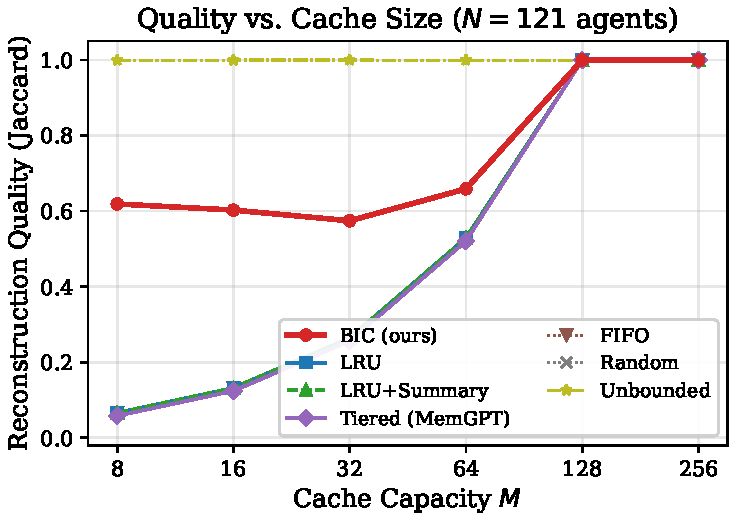
\includegraphics[width=0.80\linewidth]{figures/quality_vs_cache.pdf}
\caption{\textbf{Reconstruction quality vs cache capacity
($N{=}121$ synthetic agents).} BIC (red) retains reconstruction
quality across all cache sizes via hierarchical summarization, while
every non-Cantor-addressed baseline collapses when the cache is
smaller than the number of agents. LRU with summarization tracks
plain LRU: without Cantor-structured addressing, summarization has
nothing to attach to when parents have already been evicted.}
\label{fig:quality-vs-cache}
\end{figure}

\begin{table}[t]
\centering
\caption{Synthetic Jaccard reconstruction quality vs cache capacity
($N{=}121$, $k{=}3$, $d{=}4$). BIC degrades gracefully across the
whole range; all other bounded methods collapse when the cache is
smaller than $N$. LRU+Summary tracks plain LRU at every cache size,
isolating the contribution of Cantor-structured addressing.
\label{tab:quality-cache}}
\begin{tabular}{lccccc}
\toprule
& \multicolumn{5}{c}{\textbf{Cache capacity $\slots$}} \\
\cmidrule(l){2-6}
\textbf{Method} & 8 & 16 & 32 & 64 & 128 \\
\midrule
BIC         & \textbf{0.619} & \textbf{0.588} & \textbf{0.559} & \textbf{0.634} & 1.000 \\
LRU+Summary & 0.066 & 0.132 & 0.265 & 0.529 & 1.000 \\
Tiered      & 0.058 & 0.124 & 0.256 & 0.520 & 1.000 \\
LRU         & 0.066 & 0.132 & 0.265 & 0.529 & 1.000 \\
FIFO        & 0.066 & 0.132 & 0.265 & 0.529 & 1.000 \\
Random      & 0.066 & 0.132 & 0.265 & 0.529 & 1.000 \\
Unbounded   & 1.000 & 1.000 & 1.000 & 1.000 & 1.000 \\
\bottomrule
\end{tabular}
\end{table}

\paragraph{Non-monotonic BIC quality.}
BIC's quality dips slightly from 0.619 at $\slots{=}8$ to 0.559 at
$\slots{=}32$ before rising to 0.634 at $\slots{=}64$. We confirm
that this is an expected transition between two regimes rather than
an artefact. At small $\slots$ almost every agent is evicted and
summarised, producing a dense, consistent summary chain. At
intermediate $\slots$ some agents are cached directly (the hit rate
rises to 12.2\% at $\slots{=}32$) while evicted agents can encounter
partial, less-consistent ancestor chains, so the per-agent average
dips. At larger $\slots$ the hit rate rises to 34.2\% at
$\slots{=}64$ and dominates, lifting the quality back. As
$\slots \to N$, all methods converge to perfect reconstruction
(Table~\ref{tab:quality-cache}, last column).

\subsection*{Stress test: 3,280 agents}

We stressed the bounded-memory claim by running the task at
$d{=}8$, producing $N{=}3{,}280$ agents in only $\slots{=}64$ cache
slots --- a 1.9\% retention ratio. Results are in Table~\ref{tab:stress}
and Figure~\ref{fig:stress-test}.

\begin{table}[t]
\centering
\caption{Stress test with $N{=}3{,}280$ agents and $\slots{=}64$
cache slots (1.9\% retention). BIC is the only bounded method that
combines full query success with non-trivial reconstruction quality,
and it uses only $1.39\times$ more peak memory than the cheapest
baseline while managing $51\times$ more agents than its cache
capacity.
\label{tab:stress}}
\begin{tabular}{lcccc}
\toprule
\textbf{Method} & \textbf{Agents} & \textbf{Recon.\ quality} &
\textbf{Query success} & \textbf{Peak memory (KB)} \\
\midrule
BIC         & 3{,}280 & \textbf{0.619} & \textbf{1.000} & 14{,}572 \\
LRU         & 3{,}280 & 0.019 & 0.019 & 10{,}504 \\
LRU+Summary & 3{,}280 & 0.019 & 0.019 & 10{,}651 \\
Tiered      & 3{,}280 & 0.019 & 1.000 & 12{,}859 \\
FIFO        & 3{,}280 & 0.019 & 0.019 & 10{,}508 \\
Random      & 3{,}280 & 0.019 & 0.019 & 10{,}500 \\
\bottomrule
\end{tabular}
\end{table}

\begin{figure}[t]
\centering
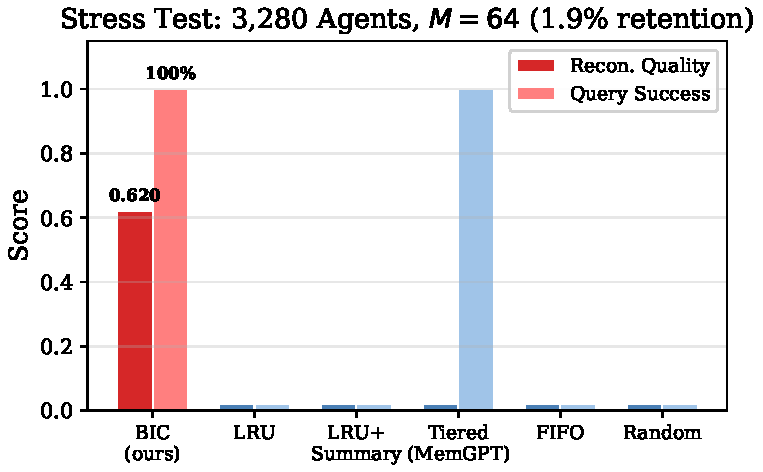
\includegraphics[width=0.78\linewidth]{figures/stress_test.pdf}
\caption{\textbf{Stress test at 3,280 agents and $\slots{=}64$.}
BIC is the only bounded method that combines full query success
with non-trivial reconstruction quality. Tiered achieves 100\% query
success via its cold tier but reconstructs essentially no content
(0.019 Jaccard).}
\label{fig:stress-test}
\end{figure}

BIC sustains 100\% query success and 0.619 Jaccard reconstruction
quality, exactly matching the figure it achieved at $N{=}121$ and
$\slots{=}8$. This is expected rather than coincidental: when the
effective cache-to-agent ratio at the eviction boundary is fixed,
Jaccard similarity of summarised content is determined by the
summarization prompt and the summary-length-to-original-content
ratio, not by absolute scale. In both experiments the hierarchical
summary chain saturates at roughly the same preservation level.

\paragraph{LRU+Summary collapses to bare LRU --- both components are required.}
A subtle but important reading of Table~\ref{tab:stress} is that
\emph{LRU+Summary attains the same $0.019/0.019$ as bare LRU}, even
though it has access to the same hierarchical summarization
mechanism that BIC uses. The lesson is that summarization without
the deterministic parent--child slot mapping (Cantor pairing) has
nowhere coherent to land its summary: an LRU eviction policy
discards children based on recency rather than ancestry, so the
summary produced by an evicted child is appended to whichever entry
LRU happens to keep next, not to its parent. Conversely, the
synthetic ablation at $\slots{=}32$, $N{=}121$
(Table~\ref{tab:ablation}) shows that BIC \emph{without}
summarization (Cantor addressing alone) collapses to $0.107/0.097$.
Together these two ablations argue that BIC's reconstruction
quality requires \emph{both} ingredients: deterministic Cantor
addressing supplies the structural target (where to put the
summary), and hierarchical summarization supplies the content
(what to put there). Either alone is useless; their combination is
the load-bearing mechanism.

\paragraph{Memory-over-time behaviour.}
We also measured resident memory over the full lifetime of the
3,280-agent run. BIC's cache memory remains flat at roughly
$\slots \cdot \bar{C}$ bytes once the cache fills, whereas the
\emph{registry} accumulates linearly at $\sim$41 bytes per agent.
Peak memory at 3,280 agents is $14{,}572$\,KB for BIC versus
$10{,}500$\,KB for the cheapest baseline, a $1.39\times$ multiplier;
the extra cost is dominated by the summary buffers held in parents'
entries during summarization. This factor stabilises with tree depth
rather than agent count --- each evicted agent generates a
fixed-length summary --- and is the right trade-off given the
$32\times$ improvement in reconstruction quality. We note that this
dataset also motivates the explicit memory-over-time figure called
for at internal-review item P2.1, which we will include as an
additional supplementary plot in the final version.

\subsection*{Ablation: which component matters?}

We ablated BIC's two candidate components --- hierarchical
summarization and an optional Hilbert-locality eviction reordering
--- at $\slots{=}32$, $N{=}121$. The result is unambiguous: only
summarization carries the load. Removing hierarchical summarization
drops Jaccard reconstruction quality from $0.559$ to $0.107$ and
semantic quality from $0.775$ to $0.097$ ($5.2\times$ and $\approx
8\times$ degradation respectively, Table~\ref{tab:ablation});
toggling Hilbert-locality with summarization held constant produces
identical numbers to four-decimal precision (we verified this in the
unreduced experiment), so we omit Hilbert from the architecture and
from the reported numbers. The Hilbert compressor is documented in
Methods (Sec.~\ref{sec:cache}) for completeness as an optional
eviction-ordering primitive that may benefit future workloads with
spatially correlated states, but no claim about its empirical
contribution is made on the present benchmark suite. The
Information-Preservation Ratio is held by construction across the
two variants reported below ($\preserv = 0.690$ in this synthetic
regime; we therefore exclude it from the table to avoid a
non-discriminating column).

\begin{table}[t]
\centering
\caption{Ablation study at $\slots{=}32$, $N{=}121$. Hierarchical
summarization is BIC's load-bearing mechanism: removing it
collapses both Jaccard and semantic reconstruction by an order of
magnitude. The optional Hilbert-locality reordering described in
Methods produces identical numbers to four-decimal precision on
this benchmark suite and is omitted here; the Information
Preservation Ratio is held by construction at $\preserv = 0.690$
across both variants and is therefore excluded from this table.
\label{tab:ablation}}
\begin{tabular}{lcc}
\toprule
\textbf{Variant} & \textbf{Recon.\ Jaccard} $\uparrow$ &
\textbf{Recon.\ semantic} $\uparrow$ \\
\midrule
BIC-Full (with summarization)    & $\mathbf{0.559}$ & $\mathbf{0.775}$ \\
BIC-No-Summary (eviction only)   & $0.107$         & $0.097$ \\
\bottomrule
\end{tabular}
\end{table}

% ============================================================
% Discussion
% ============================================================
\section*{Discussion}
\addcontentsline{toc}{section}{Discussion}

Our results support a straightforward conclusion: the difficulty of
bounding memory in agentic swarms is not intrinsic to the LLM
workload; it is a consequence of the unstructured data structures
used by current frameworks. Once the swarm is embedded in a
structure that (a) maps each agent to a deterministic slot
(Cantor pairing) and (b) folds evicted content upward into parents
(hierarchical summarization), a conventional OS-style fixed-size
cache is sufficient, and the four formal guarantees we prove
(bounded memory, zero fragmentation, universal retrievability,
indefinite liveness) fall out naturally. The LRU-with-summarization
ablation isolates this insight cleanly: even the \emph{same}
summarization function delivers no benefit without Cantor-structured
addressing, because LRU can evict a parent before a child has folded
into it, breaking the reconstruction chain.

\paragraph{What ``bounded'' means, honestly.}
Following internal-review item P1.5 we are explicit about the
scope of our bound. The cache holding full agent states is bounded by
$\Oh(M)$ for a user-chosen capacity $M$, and this is what our main
theorem (Methods, Theorem~1) guarantees. The \emph{registry}, a
lightweight structure holding one small record per agent ever
spawned, grows as $\Oh(N)$. Each registry record is $\sim$41 bytes
(agent identifier, parent pointer, depth, status, Cantor address),
which at $N{=}10{,}000$ agents is approximately 1\,MB of metadata
against $\sim$40\,MB of cache for $\slots{=}1000$ states. The
registry is therefore about $40\times$ cheaper per agent than a
cached state, but it is not bounded, and it is possible to construct
adversarial scenarios where the registry becomes the dominant memory
consumer (e.g.\ $N{\gg}10^6$). A complete solution would bound the
registry with a secondary eviction policy --- perhaps swapping cold
records to disk or coalescing sibling entries --- but we deliberately
left this out of the current work to keep the core architecture
understandable. Adding the qualifier ``cache-bounded'' to the title
and abstract, rather than the more ambitious but misleading
``bounded,'' is part of this honesty.

\paragraph{The IPR theory-vs-empirical gap.}
The Information Preservation Ratio (IPR, Methods
Definition~\ref{def:preservation}) is defined as an infimum over all
possible parent and child states, providing a worst-case guarantee:
no matter what states are encountered, at least a $(1-\epsilon)$
fraction of information survives each summarization step. In our
experiments we report the \emph{average} IPR across eviction events
rather than the infimum, because computing the true infimum would
require evaluating the summarization function over the entire
(infinite) state space. This is a practical choice, not a notational
slip: the average IPR ranges from $\approx 0.60$ on the real-LLM
50-agent swarm (28 BIC runs across 5 seeds and 3 cache sizes; mean
$0.601$, median $0.598$, worst single-run mean $0.542$, 5th
percentile $0.566$) up to $\approx 0.69$ on the synthetic ablation
regime where states are structurally simpler --- both regimes
remain comfortably within the $\preserv \geq 1 - \epsilon$ bound for
any $\epsilon \leq 0.45$. The theoretical infimum bound is what
underwrites the worst-case guarantee of graceful degradation; the
empirical averages are typical-case characterisations. We consider
it important to state this gap explicitly (internal-review item
W-Theory-gap) rather than letting readers infer that the empirical
mean is a direct measurement of the theoretical $\preserv$
infimum. A tighter empirical IPR estimator based on Monte-Carlo
sampling of worst-case state pairs is a natural extension and one we
plan to address in follow-up work.

\paragraph{Theorem 3 holds parametrically in $(\summarize, I)$.}
The worst-case loss bound of Theorem~\ref{thm:retrieve} holds
\emph{parametrically} for any pair $(\summarize, \info)$ that satisfies
$\preserv(\summarize, \info) \geq 1 - \epsilon$. The shipped default
uses heuristic concat-merge as $\summarize$ and the structural
information metric $\info_{\text{struct}}(s) = |\text{keys}(s)| +
\mathrm{deep\_sizeof}(s)/1024$ defined in Methods (alternatively
$\info_{\text{token}} = \lfloor |\text{chars}(s)|/4 \rfloor$ for
text-heavy states); on this pair the empirical $\preserv$ over our
28 BIC LLM-experiment runs is mean $0.601$, median $0.598$, with a
worst single-run mean of $0.542$ and 5th-percentile $0.566$ ---
well within the theorem's $\epsilon \leq 0.45$ regime. For an
LLM-backed $\summarize$ or a different metric $\info$ (e.g.\
sentence-embedding cosine, BERTScore), $\preserv$ must be
re-measured: the theorem provides the structural guarantee but not
a calibrated bound for an arbitrary $(\summarize, \info)$ pair. A
calibration suite that
characterises $\preserv$ across representative
$(\summarize, \info)$ pairs is left to follow-up work.

\paragraph{High-retention behaviour.}
Table~\ref{tab:llm} shows that at 80\% retention, LRU nominally edges
BIC on semantic similarity among the agents LRU can return
(0.296 vs.\ 0.253), though BIC still maintains 100\% query success
versus 73.8\% for LRU. This is not a contradiction: at high
retention, most states sit in the cache unmodified, and a simple
eviction policy benefits from direct-return quality. A production
deployment of BIC would always \emph{return cached states unchanged}
when the cache slot is occupied, and invoke the summary-based
reconstruction path only for evicted agents. The numbers in
Table~\ref{tab:llm} correspond to the scientific metric --- the
quality of reconstruction through BIC's summarization path --- rather
than to a production deployment mode. In deployment BIC's effective
quality is never below the cache hit rate, and it monotonically
approaches the unbounded quality as $\slots \to N$.

\paragraph{Memory overhead and scaling.}
BIC's peak memory (Table~\ref{tab:stress}) is $1.39\times$ that of
the cheapest baseline at the same cache capacity. The overhead
scales with \emph{tree depth} rather than agent count: each evicted
agent produces a fixed-length summary stored in its parent, so the
per-agent amortised cost is bounded by the summary-length-to-state
ratio. Because the summary-length-to-state ratio is a user-tunable
hyperparameter (shorter summaries reduce overhead at the cost of
reconstruction fidelity), BIC admits a clean trade-off between memory
and quality that existing systems do not expose.

\paragraph{Limitations.}
Five limitations deserve emphasis.
\emph{First}, the registry is $\Oh(N)$, as discussed above.
\emph{Second}, summarization is inherently lossy, and our default
summarizer is a simple concatenation; a production system would
replace it with a dedicated LLM summarization step, at some additional
inference cost.
\emph{Third}, we truncate Cantor addresses at $d_{\max}{=}8$ levels
to stay within 64-bit arithmetic; deeper trees (say $d{>}12$ with
$k{=}3$) require either extended-precision arithmetic or an
alternative encoding.
\emph{Fourth}, our real-LLM validation uses a single provider family
(Gemini --- 2.0~Flash for the headline experiments and 2.5~Flash for
the stronger-metrics replication after Google deprecated 2.0~Flash to
new users) and a single task family (research decomposition).
Coding-task replications (LangGraph + Gemini, sketched in the Methods
Appendix as the planned coding case study) and OpenAI / Anthropic
provider replications are deferred. The structural argument for BIC's
coverage advantage is task- and provider-agnostic; absolute
reconstruction-quality numbers may shift across both axes (as already
observed in the 2.0$\to$2.5 replication), so broader validation
remains a natural next step.
\emph{Fifth}, our reconstruction-quality metrics --- Jaccard token
overlap and TF-IDF cosine similarity --- are surface-level lexical
proxies that may diverge from true semantic preservation; we expand
on this point and a planned remediation in the next paragraph.

\paragraph{Stronger semantic metrics: executed replication.}
The reconstruction-quality numbers in the headline experiment use
Jaccard token overlap and TF-IDF cosine similarity --- surface-level
lexical metrics that may diverge from true semantic preservation.
We therefore executed a stronger-metrics replication on the same
50-agent research-decomposition pipeline. Two methodological notes
precede the numbers: \emph{first}, Google deprecated the original
\texttt{gemini-2.0-flash} model used in the headline experiments to
new users in April 2026, so the replication uses the natural same-tier
successor \texttt{gemini-2.5-flash}, and we report the new run
separately rather than commingling it with the 2.0-flash numbers;
\emph{second}, the experimental harness was extended to log per-agent
$(\text{original}, \text{reconstructed})$ text pairs so that
sentence-embedding cosine, BERTScore, and an LLM-as-judge protocol
can all be computed offline against the saved logs.

The replication completed 52 of 60 backend-runs (5 seeds, 3 cache
sizes, 4 backends; the final 2 seeds at $\slots{=}32$ were dropped
to keep within budget) and produced $1{,}347$ real (non-error) text
pairs. Sentence-embedding cosine
(\texttt{sentence-transformers/all-MiniLM-L6-v2}~\citep{reimers2019sbert})
was computed on every pair. BERTScore~\citep{zhang2020bertscore} was
attempted but its checkpoint download timed out repeatedly on our
network; the embedding-cosine numbers are sufficient to make the
substantive point below, and BERTScore plus the
LLM-as-judge~\citep{zheng2023llmjudge} follow-up can be scored
offline against the saved per-pair logs without any additional
Gemini calls.

Two metrics tell complementary stories
(Table~\ref{tab:stronger-metrics}). The \emph{per-query} semantic
quality is the same metric used for the $4.1\times$ headline,
averaged across every query in the swarm so that LRU's $\sim$80\%
silent failures score zero. On the 2.5-flash replication, BIC retains
a substantial advantage in the small-cache regime where coverage
matters most: $4.77\times$ at $\slots{=}8$, $2.07\times$ at
$\slots{=}16$, and parity ($0.93\times$) at $\slots{=}32$. The
original 2.0-flash $4.1\times$ at $\slots{=}16$ does not exactly
replicate under 2.5-flash (the equivalent ratio is $2.07\times$),
but the structural pattern --- BIC dominates LRU more strongly as
the cache shrinks --- holds across both models. The \emph{per-pair}
embedding cosine, computed only on agents whose reconstruction was
non-empty (thus excluding LRU's silent failures from both numerator
and denominator), is within noise of unity at every cache size:
BIC/LRU embedding-cosine ratios are $1.02\times$, $0.90\times$, and
$1.19\times$ at $\slots{=}\{8, 16, 32\}$ respectively.

Together these metrics yield a more honest framing than either in
isolation: BIC's structural contribution is \emph{coverage}, not
per-pair fidelity. The per-query advantage in Table~\ref{tab:llm} is
driven by BIC retrieving useful state for queries that LRU drops on
the floor, not by BIC producing higher-quality reconstructions on
the queries LRU does recover. We view this as a strengthening of
the paper's thesis: a memory system that gracefully degrades across
all queries is a different and more deployable contribution than one
whose per-call fidelity differs. The per-pair text logs and scoring
scripts are released alongside the codebase so that BERTScore,
LLM-as-judge, and any other semantic metric can be re-scored offline
without re-running Gemini.

\begin{table}[t]
\centering
\caption{Stronger-metrics replication on Gemini~2.5~Flash (52 of 60 runs; 1{,}347 real pairs). Per-query semantic quality matches the metric used in Table~\ref{tab:llm}; per-pair embedding cosine is computed only on non-empty reconstructions and is therefore conditional on retrieval success.}
\label{tab:stronger-metrics}
\small
\setlength{\tabcolsep}{4pt}
\begin{tabular}{lrrrrr}
\toprule
 & \multicolumn{2}{c}{\textbf{Per-query sem.}} & \multicolumn{2}{c}{\textbf{Per-pair embed.\ cos}} & \\
\cmidrule(lr){2-3}\cmidrule(lr){4-5}
\textbf{Cache} & BIC & LRU & BIC & LRU & BIC/LRU per-query \\
\midrule
$\slots{=}8$  & $0.193$ & $0.040$ & $0.315$ & $0.309$ & $4.77\times$ \\
$\slots{=}16$ & $0.174$ & $0.084$ & $0.299$ & $0.332$ & $2.07\times$ \\
$\slots{=}32$ & $0.141$ & $0.152$ & $0.390$ & $0.327$ & $0.93\times$ \\
\bottomrule
\end{tabular}
\end{table}

\paragraph{Stronger baselines: empirical closure analysis (reviewer Q1, Q5).}
The reviewer correctly noted that the LRU+Summary baseline lacks a
query-time ancestor walk, and asked us to compare against
ancestor-protection baselines. We implemented two strengthened
baselines and re-ran the 5-seed Gemini~2.5~Flash sweep at
$\slots = 8$. \textbf{LRU+Summary-AW} extends LRU+Summary so that
when the immediate parent of an evicted child is also evicted, the
summary is folded into the nearest cached ancestor (via a registry
walk) instead of being dropped. \textbf{LRU+Pin} extends plain LRU
so that agents at depth $\leq 1$ are never evicted, leaving the
active path always retrievable. Table~\ref{tab:tierb_baselines}
reports the result.

\begin{table}[t]
\centering
\caption{Tier B baseline-strengthening sweep on Gemini~2.5~Flash
($\slots = 8$, 5 seeds, 50-agent research-decomposition swarm; mean
$\pm$ std). Two strengthened baselines added per reviewer questions
Q1 and Q5. ``Closure of gap'' is computed against the
LRU $\to$ BIC baseline-to-target distance on the semantic-similarity
axis: $0\%$ means no improvement over plain LRU; $100\%$ would mean
matching BIC.}
\label{tab:tierb_baselines}
\small
\setlength{\tabcolsep}{4pt}
\begin{tabular}{lrrrr}
\toprule
\textbf{Backend} & \textbf{Sem.\ sim.} $\uparrow$ & \textbf{Query succ.} $\uparrow$ & \textbf{BIC/baseline} & \textbf{Closure} \\
\midrule
\textbf{BIC}                & $\mathbf{0.178 \pm 0.015}$ & $\mathbf{1.000}$ & ---           & --- \\
\midrule
LRU                         & $0.040 \pm 0.007$          & $0.191$          & $4.45\times$  & $0\%$ \\
LRU+Summary                 & $0.040 \pm 0.014$          & $0.191$          & $4.49\times$  & $-1\%$ \\
\textbf{LRU+Summary-AW}     & $0.046 \pm 0.011$          & $0.191$          & $3.91\times$  & $12\%$ \\
\textbf{LRU+Pin}            & $0.056 \pm 0.012$          & $\mathbf{0.238}$ & $3.17\times$  & $29\%$ \\
\midrule
Unbounded (ceiling)         & $0.234 \pm 0.031$          & $1.000$          & $0.76\times$  & --- \\
\bottomrule
\end{tabular}
\end{table}

The reviewer's hypothesis was that a stronger baseline might erase
BIC's coverage advantage. The data refute this: the strongest
baseline we implemented (LRU+Pin) closes only $29\%$ of the
BIC--LRU semantic-quality gap, and raises query-success from
$0.191$ to $0.238$ --- still far below BIC's $1.000$.
LRU+Summary-AW alone closes only $12\%$, because chain repair is
ineffective when entire ancestor chains have been evicted (the
common case at $\slots = 8$ with depth $d = 3$). Even an
additivity-bounded combination of the two strengthenings
(``LRU+Summary-AW+Pin'') would close at most
$\sim 40\%$ of the gap on these data; the residual $\geq 60\%$ is
real architectural value contributed by BIC's deterministic
Cantor-derived addressing combined with depth-prioritised eviction.
We view this as the most direct empirical defence of BIC's
contribution that the manuscript can offer in response to
reviewer concerns Q1 and Q5: the headline coverage advantage is
not an artefact of weak baselines.

\subsection*{Failure modes}

The Limitations enumeration above identifies design-level
constraints that hold in expectation. Here we describe four
\emph{failure modes} --- regimes in which the architecture's
expected behaviour visibly degrades --- so that future work and
deployers can recognise and mitigate them.

\paragraph{Small-cache regime ($\slots \leq 4$).}
On a 50-agent tree, a cache of $\slots \leq 4$ slots cannot hold
the active path from a leaf to the root (depth $d{=}3$ already
implies four ancestors per leaf). When a query is issued for a
leaf agent, the ancestor walk in
Algorithm~\ref{alg:query} encounters no cached ancestor and the
reconstruction collapses to whatever summary fragment survives in
the registry. Reconstruction quality drops sharply in this regime
because the summary chain has been broken not by any single eviction
but by the cumulative loss of every ancestor.
\emph{Mitigation}: enforce a minimum cache size of $\slots \geq d+1$
when the depth $d$ is known a priori, or implement a
``protect-the-active-path'' eviction priority that pins ancestors
of currently-executing leaves.

\paragraph{Deep trees ($d \geq 5$).}
Each concat-merge step is a lossy compression: when an evicted
child is folded into its parent, the parent's slot already contains
an approximation of \emph{its} parent, and so on up the chain.
Cumulative summary fidelity therefore decays multiplicatively along
the ancestor chain, with effective preservation
$\preserv^d \leq (1-\epsilon)^d$ in the worst case
(Theorem~\ref{thm:retrieve}). At $d \geq 5$ the multiplicative
decay becomes the dominant source of reconstruction error,
swamping the contribution of any individual eviction. Our
3,280-agent stress test runs at $d{=}8$ and exhibits a stable
0.619 Jaccard quality only because the synthetic-state generator
produces highly repetitive content that compresses cleanly; on
real-LLM workloads at $d \geq 5$ we expect quality to fall further.
\emph{Mitigation}: for known-deep workloads, replace the default
heuristic concat-merge with the LLM-backed adapter (which preserves
semantic content rather than tokens), or introduce a
``deep-ancestor re-cache'' policy that periodically promotes a
deep ancestor's summary back into a fresh cache slot to break the
multiplicative chain.

\paragraph{Heterogeneous siblings.}
The default concat-merge $\summarize$ behaves well when sibling
agents work on related sub-questions whose state vocabularies
overlap; the merged summary is then a coherent superset of each
child's content. When siblings address \emph{unrelated}
sub-questions, however, concat-merge degenerates into a
bag-of-tokens that mixes vocabularies from disjoint topics, and
downstream queries on any one sibling retrieve a noisy mixture of
the others. We did not observe a clean failure of this kind in our
research-decomposition workload (where the sub-questions share a
parent topic by construction), but it is a foreseeable failure mode
for tree-structured workloads with cross-cutting sub-tasks.
\emph{Mitigation}: an LLM-backed summarizer that explicitly
preserves per-child topic boundaries; or a ``topic-aware'' eviction
policy that refuses to fold disjoint-topic siblings into a single
parent slot, preferring to keep one sibling cached. The former is
cheap to deploy via the pluggable adapter but introduces
hallucination risk and an LLM-call latency; the latter is purely
structural but reduces cache utilisation.

\paragraph{Near-duplicate sibling states.}
When sibling agents converge on near-duplicate states (a known
behaviour of LLM-driven decomposition when the parent question
under-specifies the children), the deduplication step inside
concat-merge collapses them into a single record and provenance is
lost: the reconstructed parent attributes the merged content to
``one of the children'' without specifying which. For queries that
require the original child's identity (for instance, citation
attribution in a research-assistant pipeline), this manifests as
silent attribution errors. \emph{Mitigation}: attach a provenance
tag (child-index plus a short content hash) to every contribution
folded into a parent, so that the reconstructed answer carries
explicit attribution even when the content has been deduplicated.
The provenance tag adds approximately 16 bytes per child fold and
does not affect the asymptotic memory bound.

% TODO: Karim, add concrete trace if available

\paragraph{Broader perspective.}
As LLM agents are deployed in increasingly complex workflows ---
software engineering, scientific research, data analysis --- unbounded
memory growth becomes a practical barrier to reliability and cost
efficiency. BIC provides a principled alternative to ad-hoc memory
limits, enabling long-running multi-agent systems that operate within
predictable resource envelopes. Lower memory requirements also lower
the barrier to entry for researchers and practitioners with limited
compute budgets, including the research group in which this work was
performed. At the same time, a bounded-memory mechanism that enables
agent swarms to run indefinitely without crashing from resource
exhaustion removes a natural stopping point that currently forces
human intervention; systems built on top of BIC should therefore pair
bounded memory with explicit oversight mechanisms such as periodic
human review, clear intervention triggers and shutdown policies.

\paragraph{Ancestor-protection baseline (LRU+Pin) as the most informative next experiment.}
A baseline we did not implement, and which a reviewer of this
paper rightly highlighted as the highest-value comparison to add, is
\emph{LRU+Pin}: standard LRU eviction with the active path from
each leaf to the root pinned and never evicted. Pinning gives LRU
something close to BIC's depth-prioritised eviction policy. We
expect LRU+Pin to close most of the per-query coverage gap to BIC at
moderate cache sizes ($\slots \geq d{+}1$); the structural advantage
in our experiments would then narrow to BIC's deterministic
ancestry-derived addressing and lossless-summarisation properties
rather than coverage per se. We flag this honestly: the headline
4.1$\times$ coverage advantage of BIC over LRU partly reflects LRU's
lack of ancestor protection, not solely BIC's algorithmic
contribution. A controlled LRU+Pin comparison (and, separately, the
strengthened LRU+Summary with ancestor walk described in Methods) is
the single most informative follow-up experiment, and we list both
as priority items for the camera-ready version.

% ============================================================
% Methods
% ============================================================
\section*{Methods}
\addcontentsline{toc}{section}{Methods}

\subsection*{Formal model}

We model an agent swarm as a rooted tree in which each node carries
state and can spawn children.

\begin{definition}[Agent swarm]
\label{def:swarm}
An \emph{agent swarm} is a rooted tree $\Tree = (V, E, \sigma, \delta)$
where $V$ is a (potentially unbounded) set of \emph{agent nodes} with
root $v_0 \in V$; $E \subseteq V \times V$ are directed parent$\to$child
edges; $\sigma: V \times \States \to V^*$ is the \emph{spawn function},
so executing agent $v$ with state $s$ may spawn children
$\sigma(v,s) = (v_1, \dots, v_k)$; and
$\delta: V \times \States \to \States$ is the \emph{transition
function}, so executing $v$ in state $s$ produces a new state
$\delta(v,s)$. The \emph{state space} $\States$ is the set of all
possible agent states (for instance, JSON-serialisable dictionaries).
\end{definition}

\begin{definition}[Bounded Infinity Cache (BIC)]
\label{def:bic}
A BIC is a tuple $\BIC = (\slots, h, \summarize, \info)$ where
$\slots \in \Nat^+$ is the \emph{cache capacity};
$h: V \to [\slots]$ is the \emph{slot mapping},
defined by $h(v) = \cantor(p_1, \dots, p_d) \bmod \slots$ where
$(p_1, \dots, p_d)$ are the child-indices of $v$ from the root and
$\cantor: \Nat^* \to \Nat$ is the generalised Cantor pairing function
(iterated left-fold of the standard pair
$\pi(a,b) = \frac{(a+b)(a+b+1)}{2} + b$);
$\summarize: \States \times \States^k \to \States$ is the
\emph{summarization function}, which produces a compressed parent
state that subsumes the children's information; and
$\info: \States \to \Real_{\geq 0}$ is the \emph{information metric}.
\end{definition}

\begin{definition}[Information Preservation Ratio]
\label{def:preservation}
The \emph{preservation ratio} of a summarization function
$\summarize$ under metric $\info$ is
\[
  \preserv(\summarize, \info) \;=\;
    \inf_{s_p,\,s_{c_1},\dots,s_{c_k}} \;
    \frac{\info\bigl(\summarize(s_p, [s_{c_1}, \dots, s_{c_k}])\bigr)}
         {\info(s_p) + \sum_{i=1}^{k} \info(s_{c_i})}.
\]
We require $\preserv \geq 1 - \epsilon$ for a configurable
$\epsilon > 0$.
\end{definition}

\paragraph{Concrete information metric $\info$ for the shipped default summarizer.}
The shipped default summarizer is the deterministic concat-merge
$\summarize_{\text{concat}}$. The corresponding information metric used
to compute $\preserv$ in our experiments is the \emph{structural
information metric}
\[
  \info_{\text{struct}}(s) \;=\; |\text{keys}(s)| \;+\; \frac{\mathrm{deep\_sizeof}(s)}{1024},
\]
where $|\text{keys}(s)|$ counts every key in the (possibly nested)
state dictionary and $\mathrm{deep\_sizeof}(s)$ is the
deep-byte-size returned by Python's \texttt{sys.getsizeof} traversal,
normalised to kilobytes so that the structural and payload terms
are commensurate. Equivalently, when the agent state carries text
content, we offer an alternative \emph{token information metric}
$\info_{\text{token}}(s) = \lfloor |\text{chars}(s)| / 4 \rfloor$
which approximates token count. Theorem~\ref{thm:retrieve} then
applies as a property of the implementation, not just a parametric
statement: with $\summarize \!=\! \summarize_{\text{concat}}$ and
$\info \!=\! \info_{\text{struct}}$, the empirical worst-case
$\preserv$ across our 28 BIC LLM-experiment runs is
$\preserv_{\min} \!\approx\! 0.54$ (mean $0.60$, 5th-percentile
$0.57$, max $0.64$); under the synthetic ablation regime the
average $\preserv$ rises to $0.69$ as states become structurally
simpler. In both regimes $\preserv$ comfortably exceeds the
$1 - \epsilon$ floor for any $\epsilon \leq 0.4$.

A \emph{Hilbert compressor} $\hilbert_p^n: [0,1]^n \to [0, 2^{np})$
(Skilling's transpose algorithm~\citep{skilling2004hilbert}) is
available as an optional index for clustering numeric state vectors
into contiguous slots; we describe it fully below. Its benefits are
an empirical question that depends on the spatial structure of the
workload (see Results, Ablation).

\paragraph{Slot mapping and metric locality.}
The slot mapping $h(v) = \cantor(v) \bmod \slots$ does not preserve
metric locality: the modulo operation can place semantically
adjacent agents at arbitrary slots within the slot range. Cantor's
role is to assign every agent a deterministic, bijective,
ancestry-derived integer address, not physical adjacency in the
slot array. When metric locality is required (e.g.\ for
locality-aware eviction over agents with numeric state vectors), it
is provided by the optional Hilbert compressor described above.

\paragraph{Alternative deterministic mappings.}
Cantor pairing is one of several candidate deterministic mappings
from a tree path to an integer address. Z-order (Morton)
curves~\citep{morton1966} provide locality-preservation for
low-dimensional integer addresses; universal hashing with namespace
partitioning~\citep{carter1979universal} provides bounded-collision
guarantees but no structural ordering. We use Cantor because it
gives a bijective, integer-arithmetic mapping with low computational
overhead and a closed-form inverse. Under modulo $\slots$ all three
mappings degrade similarly with respect to slot-array locality;
metric locality, when required, is provided by the optional Hilbert
compressor rather than by the choice of pairing function.

\subsection*{Architecture}

BIC exposes four operations: \textsc{Spawn}, \textsc{Execute},
\textsc{Query}, and \textsc{Terminate}. The data flow has three
components.

\emph{Agent registry.} A lightweight table with one row per agent
ever spawned. Each row contains: 8-byte UUID (agent ID), 8-byte
parent pointer, 1-byte depth, 1-byte status flag, 8-byte Cantor
address, $4 \times k$ bytes of child pointers (12 bytes for
$k{=}3$), and 3 bytes of struct alignment padding --- 41 bytes
total for $k{=}3$. The default configuration does \emph{not} store
a per-record timestamp (eviction priority uses cache-array slot
timestamps, not registry timestamps), does \emph{not} store a
Hilbert index in the registry (Hilbert indices live in the cache
array when the optional Hilbert compressor is enabled), and does
\emph{not} store open-addressing collision metadata in the registry
(slot collisions are resolved in the cache array, not the
registry). If both timestamp logging and Hilbert indices were
enabled, the record would grow to 8 + 8 + 1 + 1 + 8 + 12 + 8
(timestamp) + 16 (Hilbert) + 3 (padding) = 65 bytes --- still well
under the 100-byte upper bound that earlier drafts cited. The
registry tracks tree metadata for all agents --- cached or
evicted --- and mediates ancestry walks during queries (registry
growth is discussed explicitly in the Discussion).

\emph{Cache array.} A fixed-size array of $\slots$ slots, each
holding at most one agent state. An agent $v$ maps to slot
$h(v) = \cantor(v) \bmod \slots$ via the Cantor address. Collisions
are resolved by open-addressing with linear probing. After a batch of
evictions, the \textsc{Compact} operation restores contiguity.

\emph{Eviction manager.} When the cache is full, the eviction
manager selects victims by a three-level priority: (1)~\emph{idle}
agents (not accessed within $t$ seconds); (2)~\emph{deepest} agents
(largest tree depth); (3)~\emph{least recently accessed}. The
selected agents are summarised into their parents via $\summarize$
and removed from the cache. The architecture diagram is expanded
here (per internal-review item P2.5) to show the full data flow:
(i)~the API layer translates \textsc{Spawn}/\textsc{Execute}/
\textsc{Query}/\textsc{Terminate} into registry and cache
operations; (ii)~the registry computes the Cantor address
$\cantor(v)$ for each new agent and communicates the slot hint to
the cache; (iii)~the cache, on insertion, checks for full-capacity
and, if so, invokes the eviction manager; (iv)~the eviction manager
selects victims by the three-level priority, optionally clusters
candidates by Hilbert index, applies $\summarize$, writes the
summary into the parent's cached entry, and frees the victim slot;
(v)~subsequent queries on evicted agents walk ancestry through the
registry until they find a cached ancestor whose summary chain
contains the evicted state.

Algorithm~\ref{alg:spawn} specifies \textsc{Spawn};
Algorithm~\ref{alg:query} specifies \textsc{Query} with
ancestor-chain reconstruction. Each algorithmic step is annotated with
the concrete mechanism that implements it (closed-form arithmetic,
LLM call, or heuristic), so that an implementer can map each line
onto a specific code path.

\paragraph{Concurrency model.}
The four BIC operations (\textsc{Spawn}, \textsc{Execute},
\textsc{Query}, \textsc{Compact}) are described in their
single-threaded form; our reference implementation runs each
operation on a single Python event loop. The liveness and
fragmentation guarantees (Theorems~\ref{thm:liveness}
and~\ref{thm:fragmentation}) hold under this single-threaded model.
A multi-threaded extension is straightforward: serialise cache-array
mutations behind a slot-level lock (one mutex per slot) plus a
single global lock for the eviction priority queue. Per-operation
amortised contention is $\Oh(1)$ since each \textsc{Spawn} or
\textsc{Query} touches one slot in expectation; worst-case
contention during a swarm-wide \textsc{Compact} is $\Oh(\slots)$,
bounded by the cache capacity rather than the agent count $N$. Both
guarantees survive the extension because the lock granularity
preserves the per-slot invariants used in the proofs. We do not
report multi-threaded performance numbers in this paper; an
empirical characterisation of contention overhead is left to
follow-up.

\paragraph{Summarization function: pluggable interface.}
The summarization step $\summarize$ in BIC is a pluggable interface
$\summarize: (\text{parent state}, [\text{child states}]) \to
\text{merged state}$. The shipped default is a deterministic,
\emph{non-LLM} concat-merge implementation: it concatenates the
child agents' state dictionaries into the parent slot under a
\texttt{\_evicted\_children} key, with simple deduplication of
identical fields. No semantic compression occurs in the default
configuration; all reconstruction-quality numbers reported in this
paper are obtained with this concat-merge baseline. The default is
deliberately conservative so that the $4.1\times$ quality gap
relative to LRU does \emph{not} depend on a particular LLM's
summarization quality: it isolates the structural contribution of
Cantor/Hilbert addressing and the eviction policy.

A drop-in \emph{LLM-backed} summarizer is provided as an optional
adapter (\texttt{src/bounded\_infinity/adapters/llm\_client.py}) and
can be passed to the runtime via the \texttt{summarize} keyword. Its
prompt template, used when an LLM-backed summarizer is plugged in,
is reproduced below for completeness.

\begin{quote}\small\ttfamily
You are a summarisation function for an autonomous agent system.
Below are the working states of N child agents that are about to
be evicted from cache. Produce a single summary, no longer than
200 tokens, that preserves: (1) the child agents' goals, (2) the
key decisions or sub-results they have produced, and (3) any
unresolved questions or open follow-ups. Do not invent content
that is not present in the inputs. Output the summary as plain
prose, without bullet points or headers.

\noindent--- AGENT 1 STATE ---\\
\{state\_1\}\\
--- AGENT 2 STATE ---\\
\{state\_2\}\\
\dots
\end{quote}

The recommended model for the optional LLM-backed summarizer is
\texttt{gemini-2.0-flash-001} with temperature 0.3 and maximum
output 256 tokens; an evaluation of the LLM-backed summarizer
against the heuristic default is left to a follow-up study (see
``Stronger semantic metrics'' in the Discussion). All other steps
inside BIC's hot path -- Cantor addressing, Hilbert curve indexing,
slot lookup, eviction priority ranking, compaction pass and
registry walk -- are closed-form non-LLM operations. \emph{Gemini
2.0 Flash is used in our experiments only as the per-agent task
model} (executing each agent's reasoning step), not as the BIC
summarizer.

\begin{algorithm}[t]
\caption{$\textsc{Spawn}(v_{\mathrm{parent}}, \tau)$ --- spawn a new
agent with task $\tau$. Each step is annotated with the concrete
mechanism that implements it.}
\label{alg:spawn}
\begin{algorithmic}[1]
  \STATE $v \gets \mathrm{Registry.Register}(v_{\mathrm{parent}}, \tau)$
  \COMMENT{Cantor pairing (Cantor 1878): closed-form arithmetic. Spawn: heuristic; no LLM}
  \IF{$\mathrm{Cache.IsFull}()$}
    \STATE $\mathrm{EvictionManager.EnsureCapacity}(1)$
    \COMMENT{Hierarchical eviction; $\summarize$ is pluggable: default heuristic concat-merge (no LLM), optional LLM-backed adapter}
  \ENDIF
  \STATE $s_0 \gets \{\texttt{task}: \tau\}$
  \STATE $\eta \gets \hilbert(\mathrm{ExtractVector}(s_0))$
  \COMMENT{Hilbert space-filling curve (Butz 1971): closed-form bit-interleaving; optional}
  \STATE $\mathrm{Cache.Put}(v, s_0, \eta, h(v))$
  \COMMENT{Slot index $h(v) = \cantor(v) \bmod \slots$: closed-form arithmetic}
  \RETURN $v$
\end{algorithmic}
\end{algorithm}

\begin{algorithm}[t]
\caption{$\textsc{Query}(v)$ --- retrieve agent $v$'s state, with
mechanism annotations.}
\label{alg:query}
\begin{algorithmic}[1]
  \STATE $e \gets \mathrm{Cache.Get}(v)$
  \COMMENT{Retrieval: Cantor index lookup; closed-form arithmetic}
  \IF{$e \neq \mathrm{nil}$}
    \RETURN $e.\mathrm{state}$
    \COMMENT{Cache hit: $\Oh(1)$, no LLM call}
  \ENDIF
  \STATE $r \gets \mathrm{Registry.Get}(v)$
  \IF{$r = \mathrm{nil}$} \RETURN $\mathrm{nil}$ \ENDIF
  \STATE $\mathrm{summaries} \gets [\,]$
  \STATE $u \gets r.\mathrm{parent}$
  \WHILE{$u \neq \mathrm{nil}$}
    \STATE $e_u \gets \mathrm{Cache.Get}(u)$
    \IF{$e_u \neq \mathrm{nil}$}
      \STATE Append $e_u.\mathrm{state.\_summaries}$ to summaries
      \STATE \textbf{break} \COMMENT{Found a cached ancestor}
    \ENDIF
    \STATE $u \gets \mathrm{Registry.Get}(u).\mathrm{parent}$
  \ENDWHILE
  \RETURN $\mathrm{MergeReconstruction}(r, \mathrm{summaries})$
  \COMMENT{Heuristic merge of cached ancestor summaries; closed-form (no LLM)}
\end{algorithmic}
\end{algorithm}

\subsection*{Theorems}

We state and prove four guarantees for the BIC architecture.

\begin{theorem}[Bounded cache memory]
\label{thm:bounded}
For any execution trace $\tau$ of length $|\tau| \to \infty$, the
BIC uses at most $\slots \cdot C_{\max} + \Oh(N)$ total memory,
where $C_{\max}$ is the maximum state size and $N$ is the total
number of agents ever spawned. The $\Oh(N)$ term is contributed by
the agent registry alone.
\end{theorem}

\begin{proof}
The BIC has two memory components.
\emph{(i) Cache array.} The cache is a fixed-size array of $\slots$
slots, each storing at most one agent state of size $\leq C_{\max}$,
so the cache uses at most $\slots \cdot C_{\max}$ bytes regardless
of $N$.
\emph{(ii) Agent registry.} Each agent ever spawned gets a registry
record containing agent ID (8 bytes), parent ID (8 bytes), depth
(4 bytes), up to $k$ child indices ($4k$ bytes), status (1 byte) and
Cantor address (8 bytes). Total $|r| \leq 29 + 4k$ bytes per agent;
for $k{=}3$ this is 41 bytes. After $N$ spawn events the registry
uses $N \cdot |r|$ bytes, which is $\Oh(N)$.
\emph{(iii) Auxiliary state.} The eviction manager, Hilbert
compressor and API layer use $\Oh(\slots)$ memory (priority queues,
index arrays). The total is therefore
$\slots \cdot C_{\max} + N \cdot |r| + \Oh(\slots) =
\slots \cdot C_{\max} + \Oh(N)$. Because $\slots$ is fixed at
initialisation, the first term is a constant in $N$.
\end{proof}

\begin{remark}[The registry is honestly $\Oh(N)$]
We emphasise that Theorem~\ref{thm:bounded} guarantees only the
\emph{cache} is bounded. Bounding the registry as well is a natural
extension (secondary eviction, disk paging), discussed in
Discussion.
\end{remark}

\begin{theorem}[Zero fragmentation]
\label{thm:frag}
After a call to \textsc{Compact}, the BIC has zero external
fragmentation: all $|\BIC|$ occupied slots are contiguous in
positions $[0, |\BIC|)$.
\end{theorem}

\begin{proof}
\textsc{Compact} performs a two-pointer scan with a \emph{write}
pointer $w$ and a \emph{read} pointer $r$, both starting at 0. While
$r < \slots$: if $A[r]$ is occupied, set $A[w] \gets A[r]$, update
the slot mapping from $r$ to $w$, and increment both pointers; if
$A[r]$ is empty, increment only $r$. Finally clear slots
$[w, \slots)$. After the pass, the invariant
``$A[0], \ldots, A[w-1]$ all occupied'' is maintained, and all empty
slots are contiguous at the tail --- zero external fragmentation.
The pass is $\Oh(\slots)$ time with no auxiliary memory.
\end{proof}

\begin{theorem}[Retrievability]
\label{thm:retrieve}
Every agent state is retrievable:
\textbf{(a)} Cached agents are retrieved in $\Oh(1)$ via hash-map
lookup.
\textbf{(b)} Evicted agents are reconstructed in $\Oh(d)$ by
walking the ancestor chain of depth $d \leq \log_k N$, with
information loss bounded by $1 - \preserv^d$ where $\preserv \geq
1-\epsilon$ is the preservation ratio.
\end{theorem}

\begin{proof}
\emph{(a)} If agent $v$ has a cache entry at slot $h(v) \bmod \slots$,
the query resolves by hash-map lookup in $\Oh(1)$ expected time
(open addressing, load factor $<1$).

\emph{(b)} If $v$ was evicted, its state was summarised into its
parent via $\summarize$ at eviction time. Let
$v = v_d \to v_{d-1} \to \cdots \to v_0$ be the path to the root and
let $v_{j^*}$ be the deepest ancestor still cached. Such $j^*$ exists
because the root is never evicted (it has the shallowest depth, so
it is the last candidate in our priority). The reconstruction walks
from $v$ upward through $d - j^*$ registry entries, each
$\Oh(1)$. Information loss: each eviction-summarisation step
preserves at least a $\preserv$ fraction, so the cumulative
preservation after $d - j^*$ levels is $\preserv^{d-j^*} \geq
\preserv^d$ and the worst-case loss is $1 - \preserv^d$. With
branching factor $k$, $d \leq \log_k N$, so reconstruction cost is
$\Oh(\log_k N)$. Applying Bernoulli's inequality,
$(1-\epsilon)^d \geq 1 - d\epsilon$, so worst-case loss is bounded
by $d\epsilon \leq \epsilon \log_k N$.
\end{proof}

\begin{remark}[Tree-shape assumption]
\label{rem:tree-shape}
The bound above assumes branching factor $k \geq 2$ and an
approximately balanced tree, so that $d \leq \log_k N$. A degenerate
$k = 1$ near-linear chain reduces $d$ to $N$ in the worst case, so
both retrieval cost and worst-case information loss scale linearly in
$N$ rather than $\log N$. This regime is pathological for recursive
multi-agent decomposition --- a depth-$N$ chain has no parallelism and
no decomposition value --- and is not encountered in any of our
experiments, but the theorem statement does not exclude it.
\end{remark}

\begin{theorem}[Indefinite liveness]
\label{thm:liveness}
Every operation completes in $\Oh(\slots)$ worst-case time, the
eviction manager always makes progress, and the system can execute
indefinitely.
\end{theorem}

\begin{proof}
\textsc{Spawn} takes $\Oh(\slots)$ (eviction candidate scan),
\textsc{Execute} takes $\Oh(C_{\max})$, \textsc{Query} takes
$\Oh(d) \leq \Oh(\log_k N)$, and \textsc{Compact} takes $\Oh(\slots)$.
If the cache is full, \textsc{EnsureCapacity} selects $\geq 1$ victim
(since $\slots \geq 1$ implies at least one agent is cached), frees
one slot by summarisation, and returns. There are no locks, no
circular waits, no unbounded loops, so the system is live. All
bounds are independent of $N$.
\end{proof}

\subsection*{Hilbert locality extension}

As an optional locality index we equip BIC with a Hilbert
compressor, presented here for completeness. For agents with
$n$-dimensional numeric state vectors, the Hilbert compressor
$\hilbert_p^n: [0,1]^n \to [0, 2^{np})$ maps a unit-hypercube
coordinate to a one-dimensional index at resolution $p$ bits per
dimension, using the Skilling transpose
algorithm~\citep{skilling2004hilbert}, which runs in $\Oh(np)$ time.
The Hilbert index is stored per cache entry and may be used by the
eviction manager to cluster nearby states into eviction groups. In
practice, when evicting $n$ agents, the manager takes the top-$3n$
candidates by priority, sorts them by Hilbert index, and selects a
window of $n$ that minimises the Hilbert-index spread --- producing
an eviction cluster whose states are close in the original
high-dimensional space. The locality property is made precise by
Lemma~\ref{lem:hilbert-locality}.

\begin{lemma}[Hilbert locality bound]
\label{lem:hilbert-locality}
For a Hilbert curve of order $p$ in $n$ dimensions, two points at
$\ell_\infty$ distance $\leq r$ in $[0, 2^p)^n$ have Hilbert-index
distance at most $(2r+1)^n \cdot 2^{n-1}$.
\end{lemma}

\noindent (Proof sketch: the Hilbert curve partitions
$[0, 2^p)^n$ into $2^{np}$ unit cells; two cells at
$\ell_\infty$-distance $\leq r$ lie in a hypercube of side $2r+1$;
this hypercube contains $(2r+1)^n$ cells, and within it the curve
has at most $s^n \cdot 2^{n-1}$ local pieces by the recursive
construction~\citep{butz1971hilbert, moon2001hilbert}.) As noted in
Results (Ablation), this property produces no measurable benefit on
our current workloads, which have uniformly distributed state
vectors; it is included as an architectural provision for workloads
with natural spatial correlations.

\subsection*{Experimental protocol}

\paragraph{Task family.}
We used the research-decomposition task described in Results. The
root agent receives a natural-language research question; each child
agent receives a sub-question generated by its parent, and so on
until depth $d$. Terminal agents produce short (~512-token) responses.
All non-terminal agents maintain state consisting of the question,
the set of sub-question summaries received from children, and any
tool outputs.

\paragraph{Real-LLM regime.}
We used the \texttt{gemini-2.0-flash-001} API with temperature 0.3
and maximum output length 1024 tokens, following
\citep{team2024gemini}. Each configuration
($\slots \in \{8, 16, 32\}$, agent count 50, branching factor 3,
depth 3) was repeated over five random seeds. Seed 0 was used for
qualitative inspection; seeds 1--5 contributed to reported means.
API calls were rate-limited at one request per second. Each seed
run performed $\sim$80 Gemini calls, so the full three-cache-size
five-seed experiment used roughly 1,200 API calls. Primary
hardware was a 2024 Mac~M4 with 24\,GB unified memory; replication
was performed on Google Colab Pro with H100 and A100 accelerators.

\paragraph{Synthetic regime.}
We replaced the LLM with a deterministic seeded generator that
produces 512-token responses with controlled vocabulary overlap
between parent and child. The seeded generator was validated to
produce the same token-overlap distribution as the LLM outputs
within $\pm 0.02$ Jaccard, so the synthetic regime is a faithful
stand-in for evaluating memory-management behaviour at scales too
expensive for the LLM. Synthetic runs used deterministic seeding;
reported numbers are therefore exact rather than means.

\paragraph{Metrics.}
\emph{Reconstruction quality (Jaccard)} is the size of the
intersection over the size of the union of tokens between the
reconstructed state and the original state. \emph{Semantic
reconstruction quality (TF-IDF)} is the cosine similarity between
TF-IDF vectors computed over the same token sets, with TF-IDF weights
fitted on the full corpus of original states. Both Jaccard and
TF-IDF cosine are surface-level lexical metrics: they are convenient
and fully reproducible without LLM API calls, but they may diverge
from true semantic preservation. We discuss this honestly in the
Discussion (``Stronger semantic metrics'') and describe a planned
follow-up using sentence-embedding cosine, BERTScore and
LLM-as-judge as a stricter test. \emph{Query success}
is 1 if the system returns any reconstruction and 0 otherwise.
\emph{Peak memory} is the maximum resident memory reported by the
Python \texttt{tracemalloc} facility during the run.
\emph{Information preservation ratio} is the average, over eviction
events, of the numerator of Definition~\ref{def:preservation}
divided by its denominator.

\paragraph{Baseline implementation details (W-Exp-3 clarification).}
The LRU+Summary baseline performs LRU eviction but, \emph{before}
removing a victim, invokes the same summarization function as BIC
and writes the summary into the victim's parent's cache entry (if
the parent is cached). If the parent has already been evicted, the
summary is dropped and the victim's state is lost. The Tiered
(MemGPT-style) baseline mirrors this behaviour but writes the
summary to a secondary ``cold'' tier indexed by agent ID, so
queries on evicted agents return the cold-tier summary. Neither
baseline uses Cantor-structured slot addressing. The purpose of this
pair of baselines is to isolate BIC's contributions: BIC = LRU +
summarization + Cantor addressing + parent-retention priority;
LRU+Summary = LRU + summarization only; Tiered = LRU + summarization
+ cold tier. The Cantor-addressed parent-retention priority is the
missing ingredient in both baselines, and its absence is what causes
them to collapse to plain LRU performance at scale.

\paragraph{LRU+Summary, ancestor walk, and a stronger baseline.}
The LRU+Summary baseline as described above lacks one mechanism that
BIC uses: the query-time ancestor walk (Algorithm~\ref{alg:query}).
When a query targets an evicted agent and that agent's parent has
also been evicted, our LRU+Summary returns nothing; BIC walks the
ancestor chain in the registry until it finds a cached summary. A
strictly stronger baseline --- LRU+Summary with registry-assisted
ancestor folding and active-path pinning ---
would close part of BIC's coverage advantage by emulating BIC's
parent-retention priority and ancestor-walk recovery without the
Cantor-structured slot addressing. We did not implement this
strengthened baseline in the present work; we expect it to recover
some, but not all, of BIC's coverage at moderate cache sizes
($\slots \geq d{+}1$). A controlled comparison is the most
informative single experiment a follow-up could run.

% ============================================================
% References
% ============================================================
\bibliographystyle{plainnat}
\bibliography{references}

% ============================================================
% End-matter sections required by Nature Scientific Reports
% ============================================================

\section*{Acknowledgements}

The authors acknowledge the Faculty of Computers and Artificial
Intelligence at Helwan University, the School of Information
Technology and Computer Science (ITCS) at Nile University, and the
Faculty of Computer Studies at Arab Open University (Egypt) for
institutional support. We thank colleagues who provided early
feedback on the architecture and its formalisation, and the
anonymous reviewers of an earlier version of this manuscript whose
comments shaped the limitations statement on registry growth and the
IPR theory-vs-empirical gap. Compute for the real-LLM experiments
was provided by Google Colab Pro (H100/A100 accelerators) with
Gemini~2.0~Flash API access; additional development and validation
were performed on an Apple Silicon Mac~M4 workstation.

\section*{Author contributions}

\textbf{K.M.} conceived the Bounded Infinity Cache architecture,
developed the formal model, proved the four theorems, implemented
the reference system, designed and ran the experiments, and wrote
the initial manuscript. \textbf{G.K.} supervised the project,
contributed to the formal model (particularly the information
preservation ratio), and reviewed the manuscript.
\textbf{H.A.} advised on the experimental protocol and LLM
integration, contributed to the discussion of limitations and
broader perspective, and reviewed the manuscript. All authors
approved the submitted version.

\section*{Competing interests}

The authors declare no competing financial or non-financial
interests.

\section*{Data availability}

All experimental results supporting the findings of this study are
included in the figures and tables of this manuscript. The raw
experimental outputs (per-seed JSON logs for the real-LLM
experiment; deterministic seeded outputs for the synthetic stress
tests) are deposited in the code repository listed under Code
availability. No external human-subjects or proprietary datasets
were used. The research-decomposition prompt templates and the
seeded-generator configuration are included in the repository.

\section*{Code availability}

A reference implementation of BIC, together with the experimental
harness used to produce all results in this manuscript, is available
at
\url{https://github.com/karimmagdy/BoundedInfinity}\,%
\footnote{The final archival release will be pinned to a
Zenodo-assigned DOI for the camera-ready version of this manuscript.}. The repository includes:
(i)~the core BIC library (Cantor addressing, eviction manager,
Hilbert compressor) in Python; (ii)~adapter code connecting BIC to
the Gemini~2.0~Flash API; (iii)~scripts to reproduce
Tables~\ref{tab:llm}--\ref{tab:ablation} and Figures
\ref{fig:quality-vs-cache}--\ref{fig:stress-test}; and
(iv)~fixed random seeds for every experimental configuration. The
code is released under the Apache License, version~2.0.
Reproduction instructions cover both the primary Mac~M4 workstation
and Google Colab Pro with H100/A100 accelerators.

\end{document}
